\label{sec:AURsec}
\begin{figure}
	\centering
	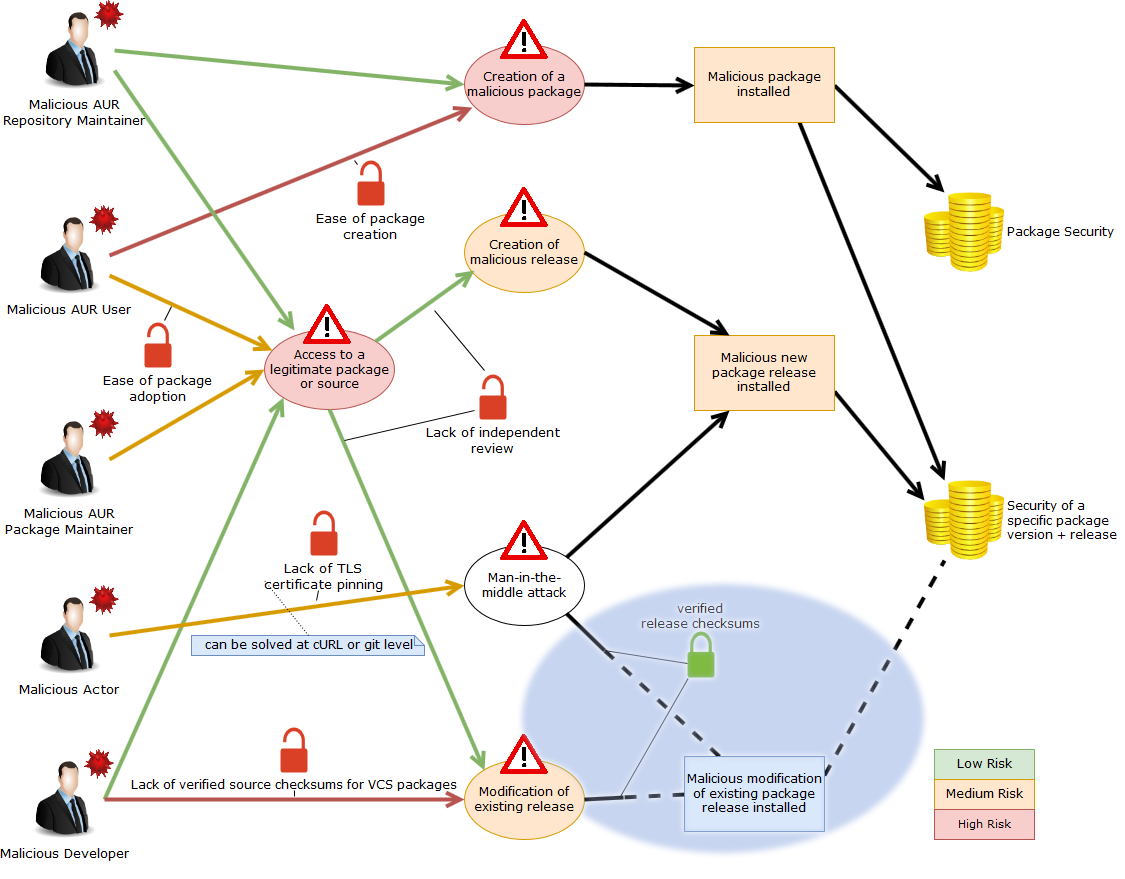
\includegraphics[width=\textwidth]{threat2n}
	\caption[Threat Prevention Strategy]{Strategy for Improving the Security of the AUR}
	\label{fig:threat2}
\end{figure}

Defence against the two attack scenarios mentioned in Section \ref{sec:attack_scenarios} requires the availability of cryptographically secure release hashes for every version of every package (Figure \ref{fig:threat2}).
If those were available, an attack would result in a hash mismatch and therefore the user could be warned.
However, the focus of the AURs design on simplicity, automation and fast package updates prevents any secure implementation on the server side as it would require the introduction of a central point of trust. That trust could only be maintained through the introduction of manual auditing, which is the opposite of what the AUR was designed for.

The solution must therefore be to implement a (preferably distributed) database on the user side, which means that there is no single authoritative source.
Since the aim is to defend against \emph{targeted} attacks, the assumption being that only comparatively few users will encounter a malicious version, this can be circumnavigated by checking the hash against a \emph{consensus} formed by many users.

% TODO: @important @lukas @bennett This paragraph is probably still unclear... need to think about that!
To make the database as safe as possible, a blockchain is used. The chain contains a smart contract providing securely callable functions. With one of these functions it is possible to commit a hash for a specific package and version.
This hash will be saved in the blockchain only if this user has not committed the same hash before, thereby making it harder to take over the blockchain and get a malicious hash to be the consensus.
The consensus is updated after every hash commit. Another function is used to get the current consensus hash and its valid commit count for a specific package and version.

This is the first project to use a blockchain as a means to provide distributed verification of (software) downloads.

% Workflow
\subsection{Workflow}
\label{sec:workflow}
The following workflow is visualized in Figure \ref{fig:main_workflow}.
\begin{figure}[!htb]
	\centering
		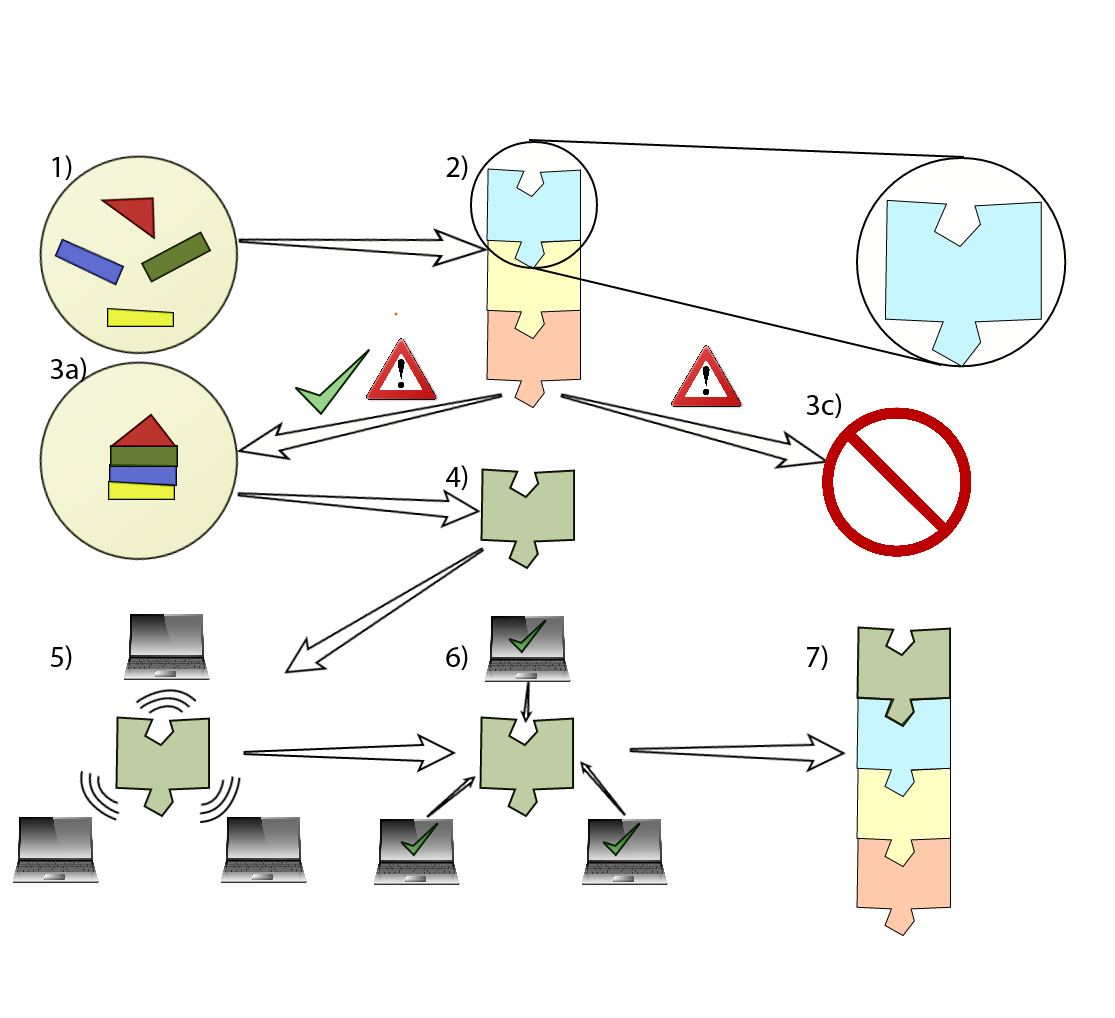
\includegraphics[width=0.6\paperwidth]{Workflow2}
	\caption{Main (Blockchain) Workflow}
	\label{fig:main_workflow}
\end{figure}

\begin{figure}[!htb]
	\centering
		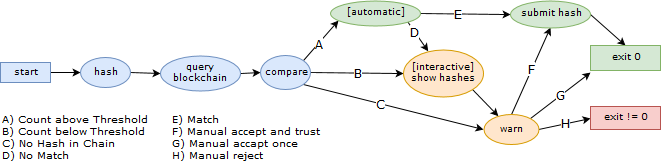
\includegraphics[width=\textwidth]{decision2}
	\caption{Aursec State Machine}
	\label{fig:state_machine}
\end{figure}


First of all a \texttt{PKGBUILD} is downloaded and partially executed in a sandbox in order to get the package version and download VCS sources (1).
Then, it is hashed along with any VCS sources and \texttt{.install} files.
The resulting local hash is compared with the current consensus (most often committed) hash of this package-version on the blockchain (2).

Depending on the comparison of the hashes (3), one of three things will happen [Figure~\ref{fig:state_machine}]:
The package may be created, installed and the hash will be added to the blockchain \emph{(Followed by step 4)} if the hashes match and the number of commits is above the trust threshold or the user decides to trust the locally generated hash anyway (A, F).

The package may be created and installed but the hash will not be added to the blockchain if the hashes do not match and/or the number is below the threshold, but the user wants to create and install the package without committing the hash. In this case the program exits with a zero status (B \rightarrow~G).

The package may not be created and installed because the hashes do not match and/or the number is below the threshold and the user doesn't want to create the package. In this case the program exits with a non-zero status (H).

If the locally generated hash is trusted, the local hash is committed to the blockchain (4). This is a transaction [see \texttt{aursec-chain commit-hash)}].
All nodes in the blockchain get the transaction over the network (5) and the transaction will be verified (together with all other transactions since the last block) and included the next mined block (6).
This mined block is then added to the blockchain (7).
As the transaction is included in a mined block, the consensus is atomically updated to reflect the new hash submission.
